% Slide 62: Online Lectures
\begin{frame}{ویدیوها و سخنرانی‌های آنلاین}{\lr{Online Lectures}}
  \begin{columns}[T]
    \begin{column}{0.58\textwidth}
      \begin{itemize}
        \setlength{\itemsep}{12pt}
        \item مطالب تکمیلی این هفته پیرامون \textbf{مقایسه عملکرد و آزمون‌های آماری مقایسه طبقه‌بندها} است.
        \item مشاهده سخنرانی‌های آنلاین و درک مفاهیم آن برای حل تمرین‌ها و موفقیت در آزمون پایانی \textbf{الزامی و حیاتی} می‌باشد.
      \end{itemize}
    \end{column}
    \begin{column}{0.40\textwidth}
      \begin{center}
        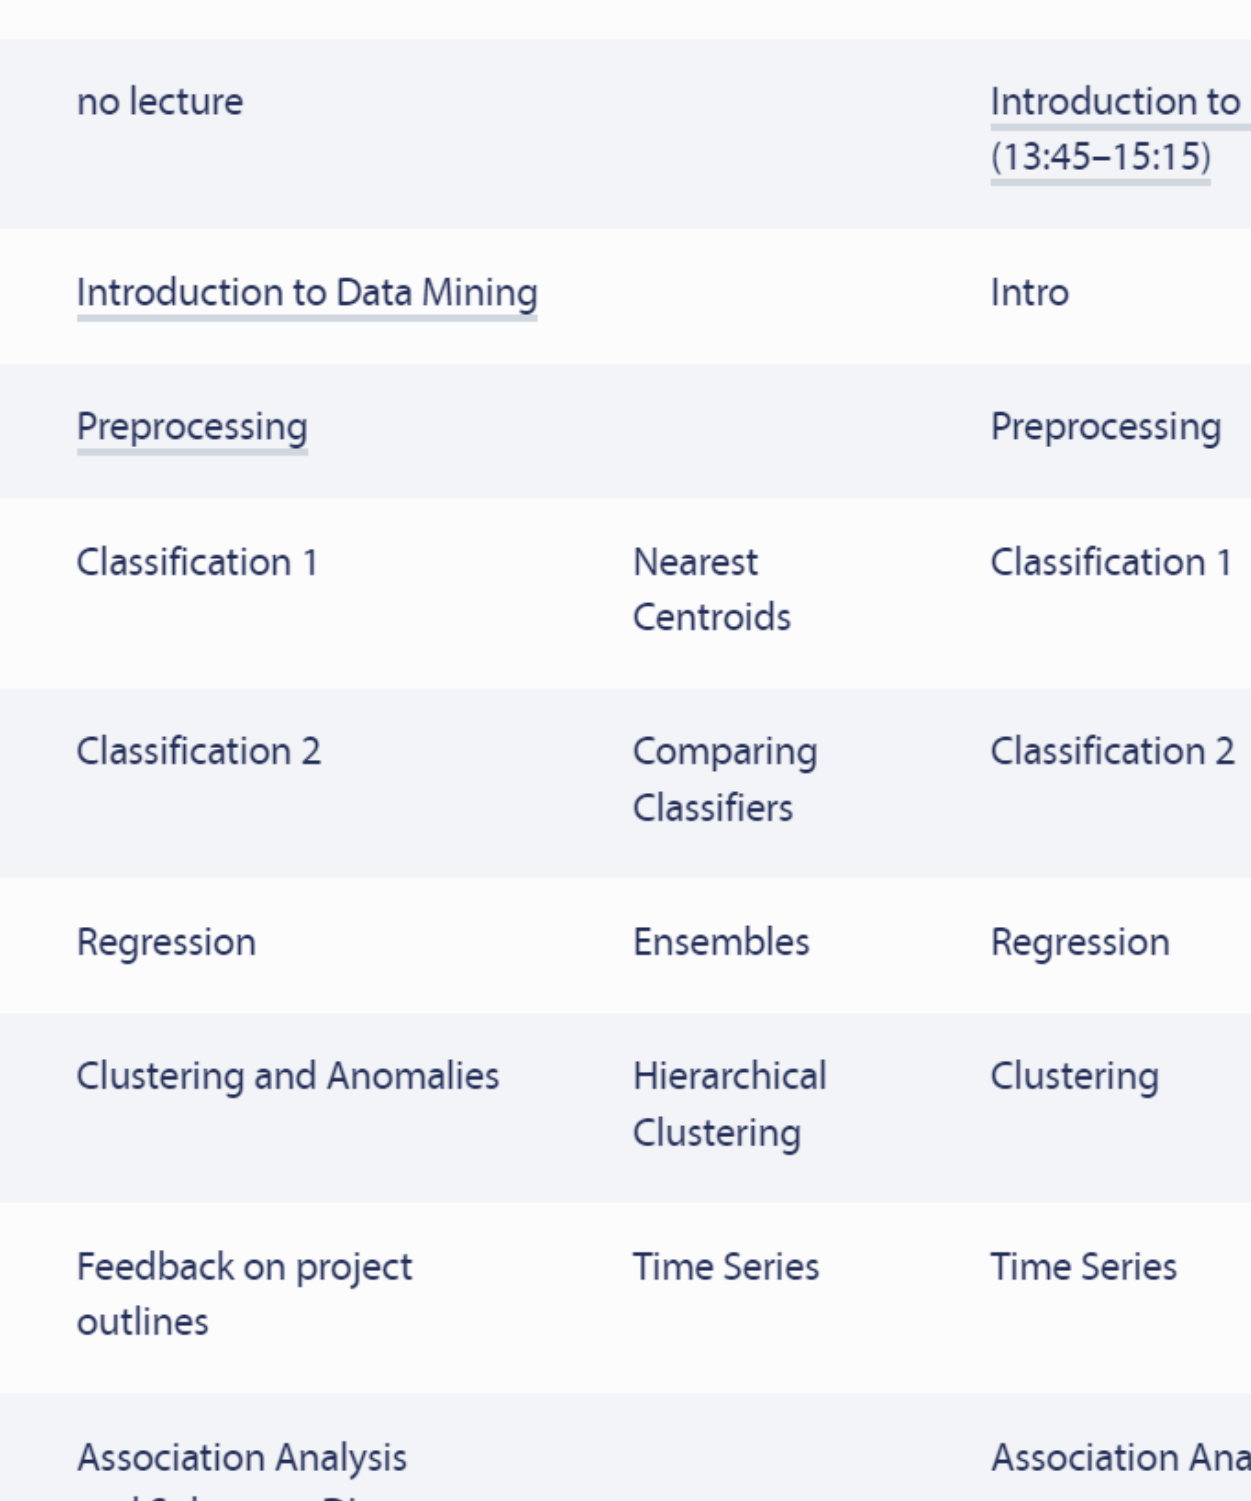
\includegraphics[width=\textwidth,height=4.8cm,keepaspectratio]{images/slide62_online_lectures.png}
      \end{center}
    \end{column}
  \end{columns}
\end{frame}

% Slide 63: Questions
\begin{frame}[plain]
  \vspace{1.5cm}
  \begin{center}
    {\fontsize{24}{28}\selectfont\color{mannheimblue}\textbf{پرسش و پاسخ}}\\[0.4cm]
    {\fontsize{13}{16}\selectfont\color{subgray}\lr{Questions \& Discussion}}\\[1.0cm]
    
\includegraphics[width=0.45\textwidth,height=3.5cm,keepaspectratio]{images/slide63_questions.png}
  \end{center}
\end{frame}

% Slide 64: Literature
\begin{frame}{مراجع و منابع این مجموعه اسلاید}{\lr{Literature \& Recommended Reading}}
  \begin{columns}[T]
    \begin{column}{0.70\textwidth}
      \begin{itemize}
        \setlength{\itemsep}{6pt}
        \item \textbf{مرجع اصلی درس:}
        \begin{latin}
          \small
          Pang-Ning Tan, Michael Steinbach, Anuj Karpatne, Vipin Kumar:\\
          \textbf{Introduction to Data Mining}, 2nd Edition, Pearson.
        \end{latin}
        \item \textbf{فصول مرتبط در کتاب مرجع:}
        \begin{itemize}
          \setlength{\itemsep}{4pt}
          \item \textbf{فصل \lr{6.4}:} بیز ساده (\lr{Naïve Bayes})
          \item \textbf{فصل \lr{6.9}:} ماشین‌های بردار پشتیبان (\lr{SVM})
          \item \textbf{فصل‌های \lr{6.7} و \lr{6.8}:} شبکه‌های عصبی (\lr{ANN})
          \item \textbf{فصل \lr{3.5}:} انتخاب مدل (\lr{Model Selection})
          \item \textbf{فصل \lr{3.7}:} حضور فراپارامترها (\lr{Hyper-Parameters})
        \end{itemize}
      \end{itemize}
    \end{column}
    \begin{column}{0.28\textwidth}
      \begin{center}
        
\includegraphics[width=\textwidth,height=5.0cm,keepaspectratio]{images/slide64_book_cover.png}
      \end{center}
    \end{column}
  \end{columns}
\end{frame}
